\chapter{Hồ sơ mô hình và kiểm toán dữ liệu}\label{pr:model-audit}

\section{Ba nhóm kết quả và mối liên hệ với Project 01 gốc}
Hệ thống trên máy demo phục vụ ba bài toán dữ liệu. Nhánh cũ có phân loại nhãn tổng hợp và hồi quy điểm tiến triển. Nhánh mới có phân loại nhị phân theo từng bộ Pima hoặc Early Stage. Cùng dùng MLP là điểm chung về họ mô hình. Các nhánh khác nhau về nguồn, biến đích, thứ tự trường và ý nghĩa đầu ra. Vì vậy, trình bày mỗi bảng kết quả cùng tên bộ dữ liệu và kích thước test.

\par\FloatBarrier\begin{table}[H]\centering\small\setstretch{1.15}\setlength{\tabcolsep}{5pt}
\caption{Kết quả test lưu từ Project 01 gốc.}\begin{tabular}{llrrll}\toprule
Tác vụ & Mô hình & Train & Test & Chỉ số 1 & Chỉ số 2\\\midrule
Phân loại & LogisticRegression & 40000 & 10000 & Acc. 0.6965 & F1 0.5005\\
Phân loại & MLPClassifier & 40000 & 10000 & Acc. 0.8180 & F1 0.5441\\
Hồi quy & Ridge & 353 & 89 & MAE 44.06 & $R^2$ 0.4791\\
Hồi quy & MLPRegressor & 353 & 89 & MAE 44.32 & $R^2$ 0.4758\\\bottomrule\end{tabular}\end{table}


Ở bài toán phân loại gốc, 7.319 trong 10.000 hàng test thuộc lớp High và 94 hàng thuộc lớp Low. MLP nhận diện đúng bảy hàng Low, tương ứng recall 7,45\%. Accuracy 81,8\% chịu ảnh hưởng lớn từ lớp High. Chênh lệch giữa accuracy và macro-F1 của mô hình gốc là ví dụ thực tế để giải thích vì sao V2 trình bày thêm recall và ma trận nhầm lẫn. Log, nhãn dự đoán và bảng theo lớp nằm trong \nolinkurl{results/per_class_metrics.json} và \nolinkurl{results/classification_predictions.csv}.

\begin{figure}[H]\centering
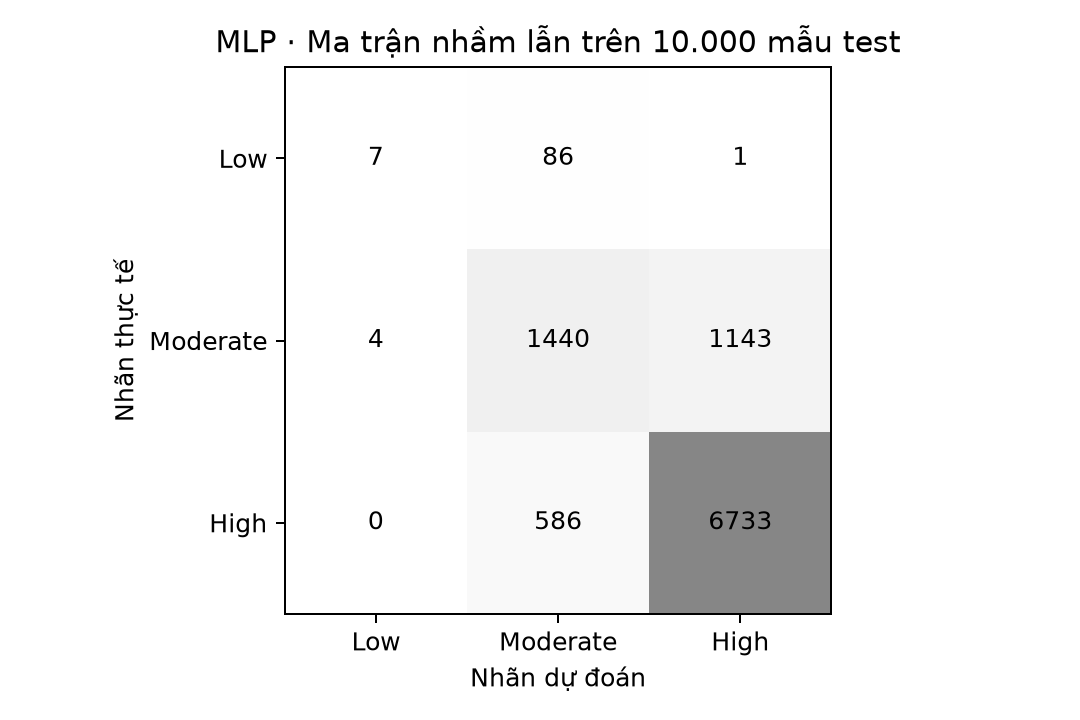
\includegraphics[width=.75\linewidth,height=.40\textheight,keepaspectratio]{../figures/confusion.png}
\caption{Ma trận của phân loại ba nhãn trong Project 01 gốc. Các số thuộc bộ 50K, lưu để đối chiếu phạm vi của từng bài toán.}
\end{figure}

Ở bài toán hồi quy gốc, Ridge có MAE 44,06 và MLP có MAE 44,32. Đích là điểm tiến triển nghiên cứu và MAE được tính theo thang điểm đó. Với từng mẫu, phần dư bằng giá trị thực trừ giá trị dự đoán. Có thể mở \nolinkurl{results/regression_predictions.csv}, đối chiếu các điểm cách xa đường chéo và tính lại MAE. Kết quả Ridge cho thấy giá trị của đối chứng đơn giản trong cùng một bài toán, tương tự vai trò của Logistic đối với V2.

\begin{figure}[H]\centering
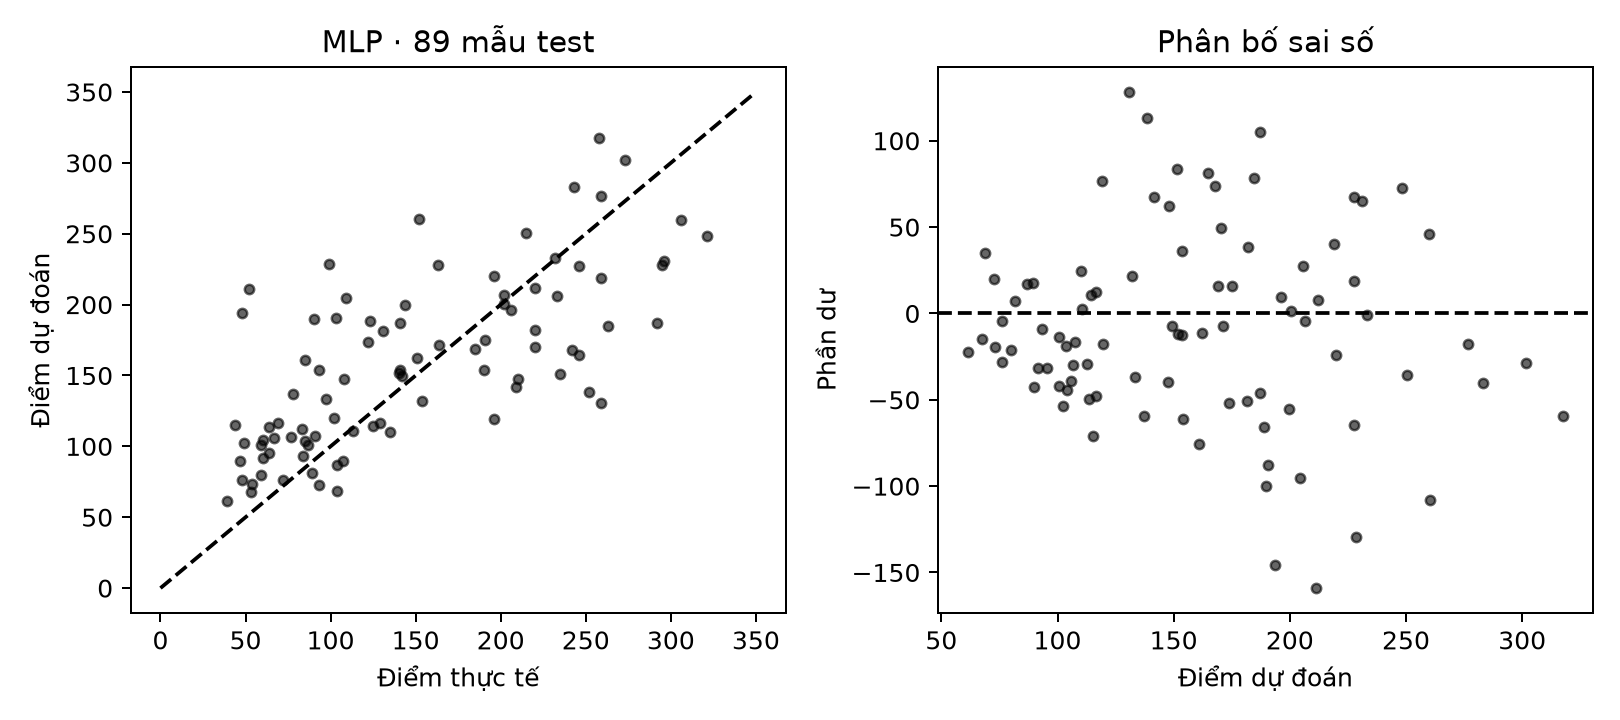
\includegraphics[width=.94\linewidth,height=.37\textheight,keepaspectratio]{../figures/regression.png}
\caption{Đối chiếu dự đoán và phần dư hồi quy của Project 01 gốc trên 89 hàng test.}
\end{figure}

\section{Từ dữ liệu thô tới hợp đồng của từng bộ}
Pima có tám đặc trưng định lượng. Một số trường đo dùng 0 như dấu hiệu thiếu. Early Stage có hai trường nhân khẩu học và 14 trường nhị phân. Trên Early Stage, nhãn Positive xuất hiện 173 lần trong 251 bản ghi sau làm sạch. Trên Pima, nhãn Positive xuất hiện 268 lần trong 768 bản ghi. Trọng số cân bằng vì thế tăng đóng góp tương đối của hai lớp khác nhau trong hai bộ.

\par\FloatBarrier\begin{table}[H]\centering\small\setstretch{1.15}\setlength{\tabcolsep}{5pt}
\caption{Từ điển 16 đặc trưng của Early Stage theo thứ tự mô hình.}\begin{tabular}{P{5.2cm}P{5.3cm}P{4.0cm}}\toprule
Trường gốc & Ý nghĩa & Dạng đầu vào\\\midrule
Age & Tuổi & Tuổi theo năm\\
Gender & Giới tính (nam=1, nữ=0) & 0 = nữ, 1 = nam\\
Polyuria & Tiểu nhiều & 0 = không, 1 = có\\
Polydipsia & Khát nhiều & 0 = không, 1 = có\\
sudden weight loss & Sụt cân đột ngột & 0 = không, 1 = có\\
weakness & Yếu sức & 0 = không, 1 = có\\
Polyphagia & Ăn nhiều & 0 = không, 1 = có\\
Genital thrush & Nấm sinh dục & 0 = không, 1 = có\\
visual blurring & Nhìn mờ & 0 = không, 1 = có\\
Itching & Ngứa & 0 = không, 1 = có\\
Irritability & Dễ cáu & 0 = không, 1 = có\\
delayed healing & Chậm lành vết thương & 0 = không, 1 = có\\
partial paresis & Yếu/liệt một phần & 0 = không, 1 = có\\
muscle stiffness & Cứng cơ & 0 = không, 1 = có\\
Alopecia & Rụng tóc & 0 = không, 1 = có\\
Obesity & Béo phì (mã dataset) & 0 = không, 1 = có\\\bottomrule\end{tabular}\end{table}

\par\FloatBarrier\begin{table}[H]\centering\small\setstretch{1.15}\setlength{\tabcolsep}{5pt}
\caption{Giá trị 0 chuyển thành thiếu trên toàn bộ Pima trước khi chia.}\begin{tabular}{lrr}\toprule
Mã trường & Số giá trị & Tỷ lệ trên 768 mẫu\\\midrule
plas & 5 & 0.7\%\\
pres & 35 & 4.6\%\\
skin & 227 & 29.6\%\\
insu & 374 & 48.7\%\\
mass & 11 & 1.4\%\\\bottomrule\end{tabular}\end{table}


Các cột có nhiều giá trị thiếu cần được giải thích khi đọc kết quả. Trên Pima, 374 giá trị insulin và 227 giá trị độ dày nếp da được đổi từ 0 sang thiếu. Trung vị dùng lúc dự đoán lấy từ tập train sau khi làm sạch. Nó là cách điền cho mô hình, không phải một phép đo mới. Ví dụ công khai trong chương minh chứng có hai trường \code{skin} và \code{insu} để trống. Có thể thấy cờ điền trung vị trong phần kết quả.

Quy tắc của API phản ánh sự khác biệt giữa giá trị thiếu và tên trường thiếu. \code{values} phải chứa đủ tên trường của dataset. Nếu một trường có tên hợp lệ và mang \code{null}, pipeline có thể xử lý thiếu. Nếu mất khóa hoặc thêm khóa ngoài schema, Data Agent báo 422. Dữ liệu nhị phân chỉ nhận mã 0 hoặc 1. Việc kiểm tra khoảng dựa trên miền quan sát của từng bộ. Registry giữ thứ tự trường cố định để một số được đưa đúng cột khi mô hình suy luận.

\par\FloatBarrier\begin{table}[H]\centering\small\setstretch{1.15}\setlength{\tabcolsep}{5pt}
\caption{Phân bố nhãn theo từng tập sau khi làm sạch.}\begin{tabular}{llrrr}\toprule
Bộ dữ liệu & Tập & Negative & Positive & Tổng\\\midrule
Pima & train & 299 & 161 & 460\\
Pima & validation & 100 & 54 & 154\\
Pima & test & 101 & 53 & 154\\
Early Stage & train & 47 & 103 & 150\\
Early Stage & validation & 15 & 35 & 50\\
Early Stage & test & 16 & 35 & 51\\\bottomrule\end{tabular}\end{table}


\section{Vì sao phải kiểm tra trước và sau khi chia?}
Trước khi chia, nhóm các hàng có cùng vector đặc trưng để tránh cùng bản ghi xuất hiện ở nhiều tập. Nếu cùng vector có nhiều nhãn, loại cả nhóm. Trường hợp giữ lại một hàng được quyết định theo thứ tự ổn định trong nguồn. Sau khi chia, kiểm tra giao của chỉ số hàng và kiểm tra trùng đặc trưng trên bộ sạch. Nếu có mã người tham gia, phép chia theo nhóm có thể tránh cùng một người có nhiều lần đo. Hai bộ hiện tại chỉ hỗ trợ kiểm tra theo bản ghi từ thông tin đang có.

Học trung vị và scaler trên tập train tạo ra một đối tượng tiền xử lý dùng lại ở validation, test và demo. Nếu tính trung vị trước phép chia, các hàng test sẽ góp vào thống kê dùng huấn luyện. Nếu refit scaler khi suy luận, cùng một giá trị sẽ có thang đo khác lúc học trọng số. Pipeline joblib chứa cả phần tiền xử lý lẫn mô hình để tránh hai lỗi này.

\section{Theo dõi một lần học và checkpoint được chọn}
Với một bộ dữ liệu và một seed, script tạo MLP theo cấu hình, tính trọng số mẫu nếu bật cân bằng rồi gọi \code{partial_fit} trên train. Mỗi epoch cho một macro-F1 validation và một log loss. Epoch có macro-F1 cao nhất được giữ. Khi bằng điểm, dùng log loss thấp hơn để chọn. Patience 60 đếm số epoch liên tiếp không cải thiện tiêu chí. Vòng train kết thúc rồi mới đo checkpoint trên test.

\par\FloatBarrier\begin{table}[H]\centering\small\setstretch{1.15}\setlength{\tabcolsep}{5pt}
\caption{Epoch được chọn theo validation và macro-F1 trên test theo từng seed.}\begin{tabular}{llrrrr}\toprule
Bộ dữ liệu & Model & Seed & Epoch & F1 validation & F1 test\\\midrule
Pima & V1 & 254 & 16 & 0.7703 & 0.7267\\
Pima & V1 & 255 & 33 & 0.7779 & 0.7351\\
Pima & V1 & 256 & 13 & 0.7550 & 0.7471\\
Pima & V2 & 254 & 5 & 0.7780 & 0.7210\\
Pima & V2 & 255 & 24 & 0.7772 & 0.7150\\
Pima & V2 & 256 & 72 & 0.7710 & 0.6587\\
Early Stage & V1 & 254 & 10 & 0.9048 & 0.8145\\
Early Stage & V1 & 255 & 5 & 0.8571 & 0.7935\\
Early Stage & V1 & 256 & 17 & 0.8417 & 0.9015\\
Early Stage & V2 & 254 & 46 & 0.9271 & 0.8741\\
Early Stage & V2 & 255 & 24 & 0.8498 & 0.9348\\
Early Stage & V2 & 256 & 18 & 0.9048 & 0.9015\\\bottomrule\end{tabular}\end{table}

\fig{figures/learning.png}{.96}{Log loss validation của V1 và V2 ở seed demo. Epoch được chọn theo macro-F1 trước, log loss dùng khi bằng điểm.}

Chẳng hạn Pima V2 seed 254 chọn epoch 5, Early Stage V2 chọn epoch 46. Hai mô hình có chung cấu hình lớp nhưng học trên dữ liệu khác nhau. Thời điểm tốt nhất còn phụ thuộc vào seed và metric chọn epoch. Bảng seed ghi kết quả từng lần chạy để người xem thấy biến thiên trước khi đọc trung bình. File checkpoint đưa vào demo thuộc seed 254, còn bảng tổng hợp lấy đủ ba seed.

\section{Phân biệt chất lượng phân lớp, xếp hạng và độ lớn của điểm}
Accuracy, recall và precision dùng nhãn sau ngưỡng 0,5. ROC-AUC mô tả khả năng xếp mẫu dương tính cao hơn mẫu âm tính qua nhiều ngưỡng. Log loss đánh giá điểm xác suất của nhãn thật và phạt mạnh khi mô hình cho điểm thấp vào lớp đúng. Một cấu hình có thể cải thiện recall ở một ngưỡng nhưng có AUC hoặc log loss xấu hơn. Khi trình bày nên đọc các số đo cùng ma trận nhầm lẫn.

\par\FloatBarrier\begin{table}[H]\centering\small\setstretch{1.15}\setlength{\tabcolsep}{5pt}
\caption{Điểm trên test ở checkpoint demo seed 254.}\begin{tabular}{llrrrrr}\toprule
Dataset & Model & Epoch & Precision + & Recall + & ROC-AUC & Log loss\\\midrule
Pima & V1 & 16 & 0.6415 & 0.6415 & 0.8154 & 0.5085\\
Pima & V2 & 5 & 0.5882 & 0.7547 & 0.8081 & 0.5315\\
Early Stage & V1 & 10 & 0.8333 & 1.0000 & 0.9875 & 0.2868\\
Early Stage & V2 & 46 & 0.8750 & 1.0000 & 1.0000 & 0.2709\\\bottomrule\end{tabular}\end{table}


Trên Pima, V2 seed demo tăng recall Positive và giảm precision Positive. ROC-AUC cũng giảm nhẹ trong lượt này. Trên Early Stage, V2 seed demo giảm số báo nhầm, giữ recall Positive bằng 1 và có ROC-AUC bằng 1 trên 51 hàng test. Số hàng test nhỏ và phép chia đã dùng trước đó giới hạn kết luận. Để thay ngưỡng cần chọn trên validation, ghi tiêu chí chọn trước khi xem test và báo lại precision, recall, ma trận và phạm vi dữ liệu.

\section{Đọc bằng chứng từ model tới bảng kết quả}
Trong \nolinkurl{results/v2/experiment.json}, tìm bộ dữ liệu, phiên bản, seed 254, epoch và hash. Áp ngưỡng 0,5 lên cột điểm tương ứng trong CSV test để đếm lại \(TN,FP,FN,TP\). Lượt API trên mẫu công khai xác nhận demo chạy model. Đối chiếu từng hàng test xác nhận model khớp với bảng kết quả.

\chapter{Vận hành agent, xử lý lỗi và dấu vết}\label{pr:failure}

\section{Các cổng vào phục vụ những thao tác nào?}
\begin{table}[H]\centering\small\setstretch{1.12}
\caption{Hợp đồng ở cấp tính năng.}
\begin{tabular}{P{4.1cm}P{5.4cm}P{4.7cm}}\toprule
Đường gọi & Vai trò trên giao diện & Dữ liệu kiểm tra\\\midrule
\code{GET /api/v2/study} & Tạo form, danh sách phiên bản và bảng so sánh & Registry, cấu hình, metric và số tầng\\
\code{POST /api/v2/predict} & Chạy mẫu qua hệ đa agent nghiên cứu & Điểm, nhãn, trace, nguồn, audit\\
\code{POST /api/chat} & Hỏi kiến thức hoặc chạy bài toán cũ & Nội dung, nguồn, chế độ sinh và trạng thái graph\\
\code{GET /api/graph} & Mở và lọc đồ thị trên web & Cạnh lấy từ Neo4j và mã đoạn\\
\code{GET /api/source/...} & Mở tài liệu được lưu trong thư viện & Tệp local được đối chiếu theo provenance\\
\code{GET /api/status} & Xem hệ thống và kiểm tra sẵn sàng & Neo4j, local LLM và cờ local-only\\\bottomrule
\end{tabular}
\end{table}

Màn hình V2 đọc metadata từ API. Việc đổi phiên bản chủ yếu đổi khóa checkpoint. Việc đổi dataset đổi cả form, tập trường và khóa checkpoint. Form định lượng dùng số và form nhị phân dùng mã. Backend vẫn xác thực lại sau khi nhận JSON vì kiểm tra ở trình duyệt có thể bị bỏ qua trong API call trực tiếp.

\section{Dấu vết của một lượt chạy bình thường}
Một yêu cầu sinh một bus riêng. Coordinator gọi sáu vai trò theo thứ tự. Bus ghi REQUEST, gọi handler rồi ghi INFORM nếu handler hoàn thành. Nếu handler ném lỗi, bus ghi FAILURE và truyền lỗi lên. V2 thêm mã yêu cầu, phiên bản, trạng thái và thời gian vào mỗi thông điệp. Hai thông điệp của một lời gọi cùng mang một thời gian đo. Khi đối chiếu chi phí, lấy một giá trị mỗi cặp.

\par\FloatBarrier\begin{table}[H]\centering\small\setstretch{1.15}\setlength{\tabcolsep}{5pt}
\caption{Một lượt Pima V2 đã lưu. Mỗi hàng là một lời gọi.}\begin{tabular}{llrr}\toprule
Vai trò nhận & Loại yêu cầu & Thời gian (ms) & Thông điệp kết quả\\\midrule
Data & REQUEST & 0.017 & INFORM\\
Prediction & REQUEST & 1.710 & INFORM\\
Rule & REQUEST & 0.005 & INFORM\\
KG/RAG & REQUEST & 7.305 & INFORM\\
Explanation & REQUEST & 0.009 & INFORM\\
Monitoring & REQUEST & 0.194 & INFORM\\\bottomrule\end{tabular}\end{table}


Prediction nhận feature order và giá trị từ Data. Rule nhận dataset và trạng thái trường thiếu. KG/RAG nhận câu hỏi đi kèm, trả đoạn và cạnh đã kiểm tra. Explanation nhận ba nhóm kết quả để trình bày phạm vi và căn cứ. Monitoring nhận metadata đã trích từ lượt chạy và ghi một dòng JSONL. Một người xem có thể dò theo mã lượt, nhận diện checkpoint qua hash và tìm lại mã đoạn tri thức.

\section{Phân biệt phản hồi lỗi và phản hồi giảm tính năng}
\begin{table}[H]\centering\small\setstretch{1.12}
\caption{Các nhánh kiểm thử theo tình trạng đầu vào và dịch vụ.}
\begin{tabular}{P{4.0cm}P{5.2cm}P{5cm}}\toprule
Tình huống & Xử lý & Dấu hiệu trên đầu ra\\\midrule
Yêu cầu hợp lệ & Thực hiện sáu lời gọi chuyên trách & Dự đoán, nguồn, trace và audit\\
Sai tập trường hoặc số không hữu hạn & Data báo lỗi trước Prediction & HTTP 422, mã yêu cầu và trace lỗi\\
Câu hỏi ưu tiên an toàn & Nhánh ưu tiên chạy trước schema và model & Không có kết quả model, audit ghi bỏ qua\\
Neo4j gián đoạn & Giữ đoạn văn bản đã tìm, trả graph unavailable & Nguồn văn bản còn, danh sách cạnh rỗng\\
Không ghi được audit & Monitoring trả trạng thái lưu thất bại & Kết quả còn, trường stored bằng false\\\bottomrule
\end{tabular}
\end{table}

Trường hợp sai dữ liệu có thể thử bằng cách xóa một khóa khỏi JSON trong kiểm thử, thay vì sửa số trên form rồi đoán backend nhận được gì. Trường hợp Neo4j gián đoạn trong test dùng driver giả lập lỗi để kiểm đúng nhánh mà không làm dừng dịch vụ demo. Lỗi checkpoint hiện cần xem log vận hành nếu pipeline không nạp được. Một bản triển khai phục vụ nhiều người cần chuẩn hóa thông báo lỗi checkpoint và đo thêm hành vi khi dịch vụ quá tải.

\section{Audit, trace và giới hạn lưu trữ}
Trace phục vụ gỡ lỗi và minh họa tương tác. Nó nằm trong phản hồi, có thể chứa giá trị đầu vào. Audit là tệp JSONL chỉ lưu metadata như request ID, phiên bản, hash, trạng thái, thời gian và mã nguồn. Hai loại dữ liệu có mục đích và vòng đời khác nhau. Khi dùng máy cá nhân để thuyết trình, lấy mẫu công khai và dùng mã yêu cầu trong ảnh để đối chiếu. Khi chuyển môi trường, cần quyết định ai được xem trace, giữ nhật ký bao lâu và cách xóa.

\section{Trình tự vận hành trên Mac}
Launcher kiểm tra mô hình GGUF, chương trình llama-server và Neo4j trước khi bật. Neo4j phục vụ giao diện Browser ở cổng 7474 và kết nối Bolt ở 7687. Sau khi Neo4j sẵn sàng, script nạp graph từ KB theo lệnh MERGE. Tiếp theo llama.cpp nạp Qwen3 4B ở 11435, rồi FastAPI chạy ở 8765. Status kiểm tra các dịch vụ và báo sẵn sàng. Dịch vụ local dùng địa chỉ loopback. Nếu chỉ cần xem báo cáo và kiểm chỉ mục, dùng truy vấn snapshot offline ở chương sau.

\begin{Verbatim}[fontsize=\small]
bash run-macos.sh status
bash run-macos.sh start
bash run-macos.sh stop
\end{Verbatim}

Khi gặp lỗi khởi động, đọc trạng thái để xác định thiếu Neo4j, Qwen hay web. Mỗi tiến trình do launcher quản lý có log trong \nolinkurl{.runtime/}. Web có thể báo Neo4j chưa kết nối dù trang tải được. Khi đổi model hoặc mã backend, khởi động lại để xóa cache checkpoint. Chạy từ thư mục project để launcher tìm đúng tài nguyên và môi trường Python riêng của dự án.

\chapter{Kiểm chứng nguồn tri thức và chỉ mục truy xuất}\label{pr:source-audit}

\section{Từ tài liệu gốc tới một đoạn có thể kiểm tra}
Một đoạn trong KB có mã tài liệu, tiêu đề, chủ đề, từ gợi ý, văn bản đã biên soạn và mã nguồn. Đoạn có provenance còn ghi nhà xuất bản, vị trí, trích đoạn ngắn và mã băm tệp. Ví dụ \code{pdf_self_management} liên kết tới PDF NIDDK, trang PDF vật lý 27, mục \emph{What is self-management?}. Có thể mở trang ngay từ thư viện, đối chiếu đoạn căn cứ rồi xem hai dạng của nguồn trong giao diện: đường dẫn trang gốc và bản lưu local.

Tệp \nolinkurl{data/source_curation.json} ghi chỉ dẫn biên soạn. Script \nolinkurl{scripts/build_sourced_kb.py} đọc nguồn lưu, kiểm trích đoạn và tạo JSON tri thức đã biên soạn. Khi khởi động, \code{app/retrieval.py} hợp nhất kho cơ sở, kho hội thoại và phần biên soạn, rồi kiểm trùng mã đoạn. Việc cập nhật tài liệu diễn ra ở bước chuẩn bị kho. Người dùng đặt câu hỏi vào dữ liệu đã được chuẩn bị.

\begin{figure}[H]\centering
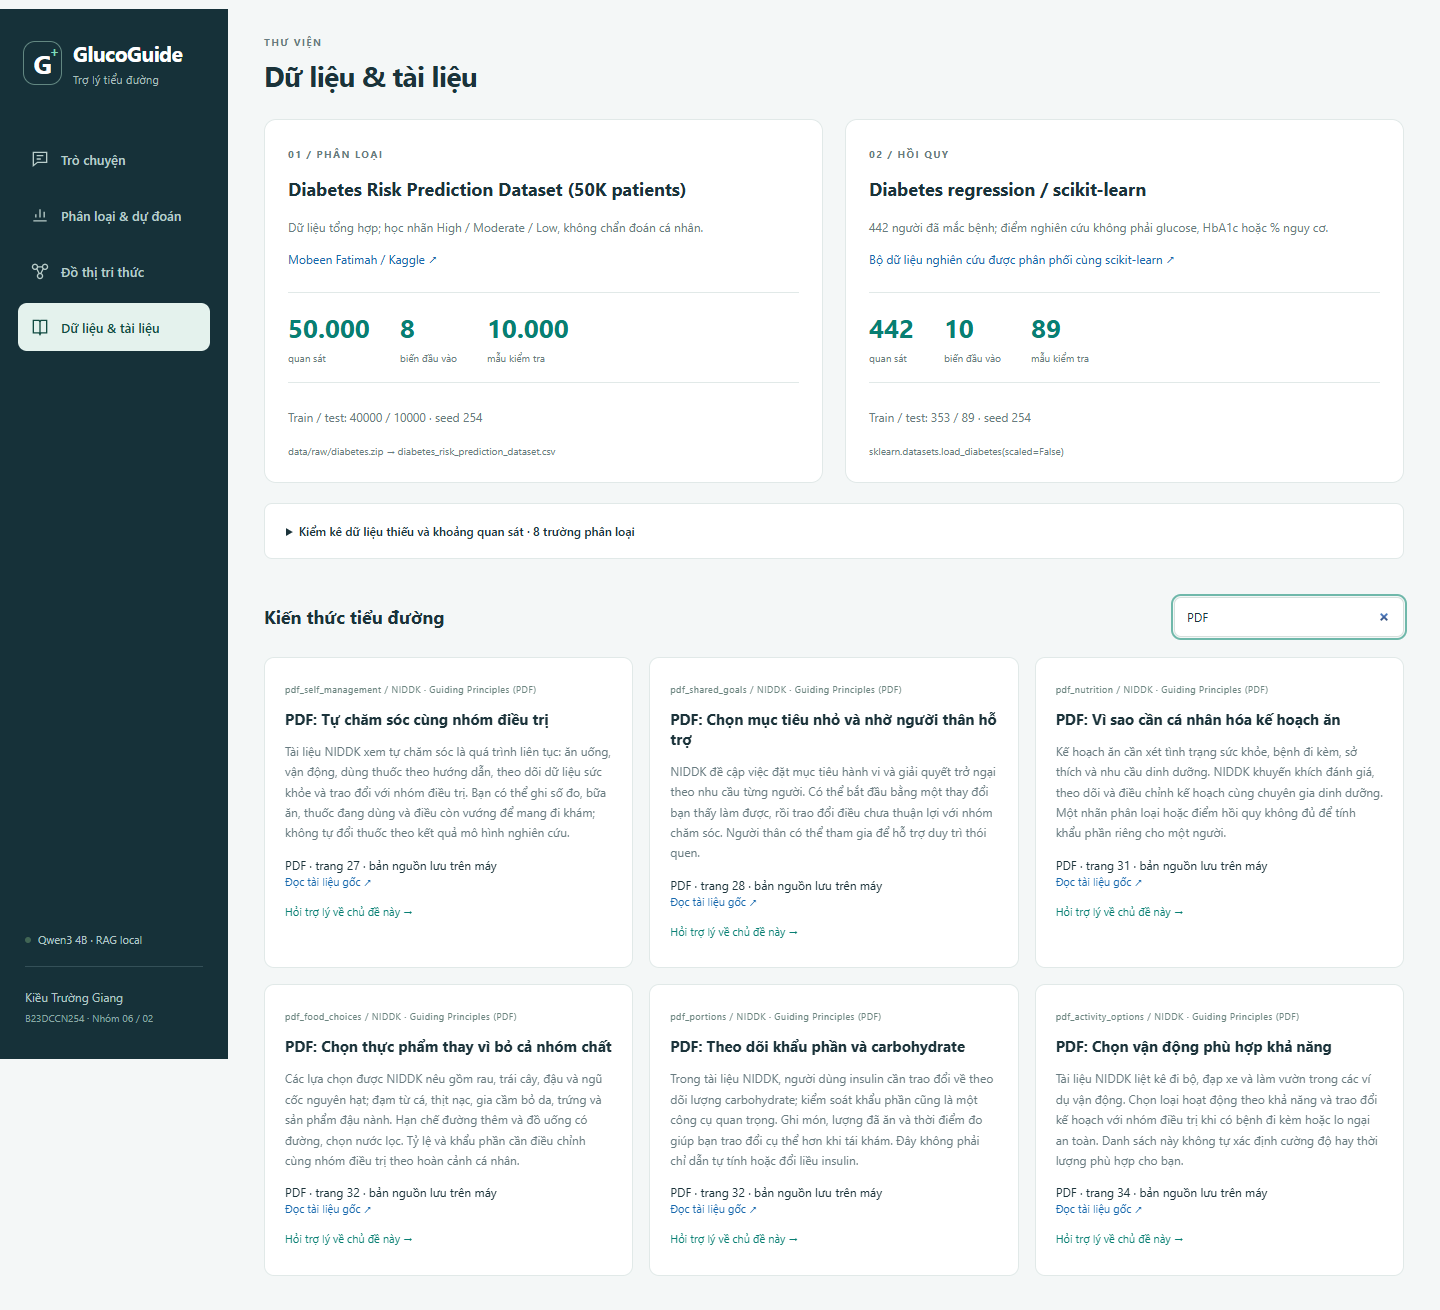
\includegraphics[width=.95\linewidth,height=.47\textheight,keepaspectratio]{../demo-pdf-sources.png}
\caption{Ảnh kiểm thử thư viện của bản local đã lưu. Các thẻ PDF hiển thị mã đoạn, trang vật lý và nút mở tài liệu gốc.}
\end{figure}

Để đối chiếu bằng mã, dùng GET \nolinkurl{/api/source/pdf_self_management}. Backend chỉ trả file đã biết trong thư mục nguồn và có provenance. Phần kiểm thử đối chiếu trang vật lý, trích đoạn và hash; khi nguồn không có bản lưu, giao diện dùng URL. Neo4j lưu cạnh gắn document ID, nên mã đoạn cung cấp đường nối từ hình đồ thị về nội dung gốc.

\section{Từ câu hỏi tới danh sách nguồn}
Bộ lập kế hoạch nhận câu hỏi và lịch sử, xác định chủ đề và có thể chỉ định danh sách nguồn cố định. Nếu đi qua xếp hạng, hệ thống dùng điểm TF-IDF từ và ký tự. Phần điểm nền có dạng
\[
  s_{\rm base}(q,d)=0{,}55\,s_{\rm word}(q,d)+0{,}45\,s_{\rm char}(q,d).
\]
Sau đó, chương trình cộng điểm theo cụm từ và mã chủ đề, loại các nguồn trái với bộ lọc yêu cầu, rồi sắp giảm dần. Một đoạn trong danh sách tối đa bốn đoạn phải vượt ngưỡng tuyệt đối 0,15 và ngưỡng tương đối \(0{,}58\,s_{\max}\). Nếu ngay điểm lớn nhất cũng thấp hơn ngưỡng tuyệt đối, xếp hạng trả danh sách rỗng.

Cụm từ đúng có thể mang thông tin tốt hơn các từ rời, còn n-gram ký tự hỗ trợ một số khác biệt nhỏ về cách viết. Điểm truy xuất dùng để sắp đoạn. Điểm cao chưa đủ chứng minh đoạn giải đáp mọi ý trong câu hỏi. Với chủ đề có nguồn cố định, danh sách được chọn theo định tuyến. Neo4j nhận tối đa bốn mã tài liệu để lấy cạnh.

\section{Đọc trường hợp nguồn kỳ vọng nằm dưới hạng một}
Bộ kiểm tra có 20 câu với nguồn kỳ vọng và hai câu không cần truy xuất. Hit@1 đạt 17/20, Hit@4 đạt 20/20. Ba câu có nguồn kỳ vọng ở hạng 2, 2 và 3. Vì vậy MRR@4 được tính là
\[
 \frac{17+1/2+1/2+1/3}{20}=0{,}9167.
\]
Bảng dưới cho thấy lý do phải đọc danh sách truy xuất. Ở ca \code{rice}, đoạn đúng có mặt nhưng đứng thứ ba, sau hai đoạn cùng chủ đề. Hai ca danh sách rỗng được xét bằng logic bỏ qua nguồn, không góp vào mẫu số 20.

\par\FloatBarrier\begin{table}[H]\centering\small\setstretch{1.15}\setlength{\tabcolsep}{5pt}
\caption{Các ca nguồn kỳ vọng xuống hạng và các ca bỏ qua truy xuất.}\begin{tabular}{lP{4cm}P{6cm}r}\toprule
Ca & Mã kỳ vọng & Kết quả đã lưu theo thứ tự & Hạng đầu\\\midrule
rice & rice\_portion, carb & web\_portion\_choices, meal\_example, rice\_portion & 3\\
foot & foot\_care & vinmec\_foot\_check, foot\_care & 2\\
drinks & drinks & monitor, drinks, overview, pdf\_self\_management & 2\\
outside & -- & -- & --\\
greeting & -- & -- & --\\\bottomrule\end{tabular}\end{table}


Bộ nguồn PDF/Vinmec gồm tám câu chức năng có mã nguồn kỳ vọng riêng. Kết quả đã lưu là tám trên tám ở hạng một. Câu hỏi được soạn để kiểm các nguồn cụ thể. Đánh giá rộng hơn cần cách diễn đạt tự nhiên đa dạng, nhiều người gắn nhãn đoạn phù hợp và nhóm câu thiếu căn cứ.

\section{Đối chiếu cạnh trước khi dùng trong prompt}
Truy vấn Neo4j lấy cạnh theo \code{r.document IN \$ids}. Sau khi lấy record, bộ lọc tìm đoạn tương ứng trong KB, kiểm chủ thể, quan hệ, đối tượng, đoạn evidence và URL. Nó loại bản ghi sai căn cứ và loại lặp. Nếu nhiều đoạn cùng trả cạnh, bộ lọc luân phiên giữa các đoạn để một nguồn không chiếm toàn bộ ngữ cảnh. Kết quả được đưa vào prompt dưới dạng các bộ ba có mã tài liệu, giúp người xem đối chiếu trích dẫn.

Các bài kiểm thử đã thay URL, văn bản, quan hệ và document ID để xác nhận fact sai bị loại. Kiểm tra khác xác nhận các đoạn văn bản đã tìm còn khả dụng khi driver báo lỗi. Khi Neo4j phục vụ bình thường, dữ liệu đối chiếu lưu tại \nolinkurl{results/graph_coverage.json} cho biết 58 trên 58 chủ đề có quan hệ được kiểm tra và tổng số cạnh là 106.

\section{Phát lại bản xuất và kiểm tra toàn vẹn}
Bản xuất chứa JSON KB, CSV/JSON graph, tệp Cypher, chỉ mục TF-IDF, cấu hình và câu hỏi kiểm tra. Script query xác minh manifest trước khi nạp index. Bản snapshot đọc quan hệ từ JSON và dùng cùng luật đối chiếu, nên có thể kiểm kết quả truy xuất offline. Nó giúp xác định lỗi thuộc bộ xuất hay dịch vụ Neo4j. Khi demo yêu cầu kết nối thật, mở trạng thái Neo4j trên web và chạy một truy vấn MATCH ở Browser.

\begin{Verbatim}[fontsize=\small]
.venv/bin/python scripts/query_knowledge_export.py \
  exports/diabetes --question "HbA1c là gì?"
\end{Verbatim}

Khi muốn dựng lại graph local từ bộ xuất, dùng \nolinkurl{scripts/restore_knowledge_export.py}. Script kiểm manifest, tạo ràng buộc tên Concept duy nhất và gọi MERGE. Bộ kiểm tra xuất kiểm tám điều kiện, trong đó có hash, dữ liệu UTF-8, tái hiện 22 ca và cú pháp Cypher. Tệp \code{kb_diabet.cypher} cấp ngoài là bản để mở nhanh khi trình bày.

\chapter{Hội thoại cục bộ, kiểm chứng và giới hạn}\label{pr:chat-control}

\section{Giữ vai trò của MLP và Qwen rõ ràng}
Prediction Agent dùng MLP nhận dữ liệu bảng có thứ tự cột để tính điểm. Qwen nhận văn bản ngữ cảnh ở luồng Trò chuyện và sinh bản nháp trả lời. Nhánh thực nghiệm V2 dùng Explanation dạng mẫu để người xem nhìn rõ điểm, cờ luật và nguồn. Qwen local là Qwen3 4B lượng tử hóa Q4\_K\_M qua llama.cpp trên Mac. Tách mô hình và đường gọi giúp thử độc lập chất lượng phân lớp, độ phủ nguồn và chất lượng nội dung.

\section{Thứ tự chọn nhánh trên một lượt hỏi}
Backend phân loại an toàn trước. Với lượt cần ưu tiên, hệ thống chọn nhánh bảo vệ và trả ngay. Khi yêu cầu thông thường, định tuyến dựa vào câu hỏi và lịch sử. Lượt hỏi tiếp có thể cần phân giải tham chiếu trước khi truy xuất. Câu hỏi đủ căn cứ nhận danh sách đoạn và cạnh đã đối chiếu. Nếu điều kiện sinh được thỏa, Qwen nhận câu hỏi đã chuẩn bị cùng ngữ cảnh. Với chủ đề có bảo vệ hoặc thiếu nguồn, hệ thống có thể trả văn bản đã biên soạn hoặc hỏi làm rõ.

Trong luồng cũ, tùy chọn nhận xét mô hình có thể gửi lại thông tin bài toán và giá trị của mẫu vừa chạy. Backend tính lại dự đoán, gắn phạm vi của bộ dữ liệu và chuyển cho phần hỗ trợ có nguồn. Điều này bảo đảm nội dung nhận xét gắn với kết quả thực nghiệm. Nếu người dùng chuyển chủ đề, câu hỏi hiện tại vẫn là căn cứ định tuyến. Lịch sử và context model có mục đích riêng.

\section{Kiểm bản nháp trước khi hiển thị}
Prompt chứa mã nguồn được phép dùng. Bộ kiểm chứng tìm mã lạ, số liệu vắng trong đoạn nguồn và các mẫu văn bản vượt phạm vi. Nó kiểm lại cạnh trước khi chấp nhận bản nháp. Nếu lượt đầu không đạt, đường gọi llama.cpp có thể thử sửa một lần. Nếu vẫn không đạt, dùng phương án KB đã chuẩn bị. Sau đó web hiển thị nguồn để người dùng đối chiếu. Kiểm tra cú pháp dẫn nguồn và số liệu là bước giảm lỗi. Mệnh đề đúng về hình thức vẫn cần được đọc cùng tài liệu để xác nhận ý nghĩa.

\section{Thử nghiệm adapter của bản gốc và quyết định triển khai}
Project 01 gốc ghi một thử nghiệm tinh chỉnh LoRA trên Qwen3 1.7B. Bộ thử đó có 76 mẫu train, 21 validation và 16 test. Hạng LoRA là 8. Có khoảng 1,61 triệu tham số được tối ưu. Qua ba epoch, loss validation tốt nhất trong tập nội bộ là 0,0082. Kết quả dùng để so định dạng và bám nguồn trong phạm vi thử nghiệm. Tập nhỏ và cùng quy trình biên soạn làm số loss khó suy rộng sang hội thoại tự do.

\begin{figure}[H]\centering
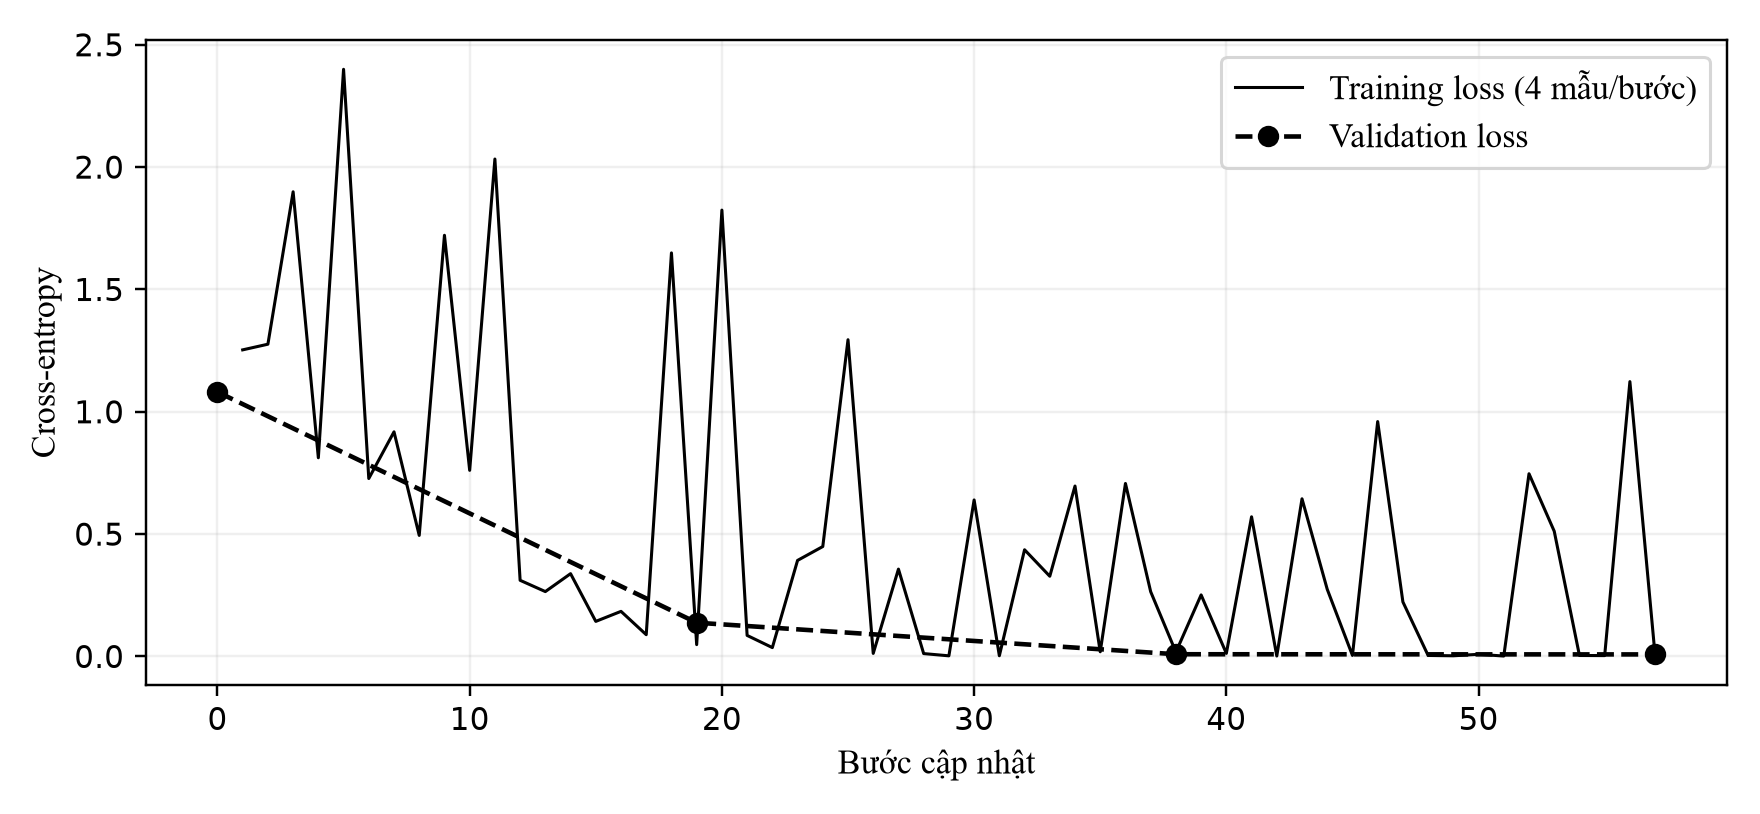
\includegraphics[width=.95\linewidth,height=.38\textheight,keepaspectratio]{../figures/qwen_learning.png}
\caption{Đường học được lưu từ thử nghiệm LoRA 1.7B của Project 01 gốc. Bản demo Mac dùng Qwen3 4B qua llama.cpp.}
\end{figure}

Quyết định dùng 4B kết hợp RAG phục vụ hệ thống hiện tại. Bảng 1.7B và các tệp trong \nolinkurl{results/local_qwen/} ghi lại quyết định đó. Trong demo, có thể đối chiếu trường \code{response_mode}, mã nguồn và thông điệp kiểm chứng ở trace. Không dùng loss của adapter để mô tả độ đúng của Qwen 4B.

\section{Đánh giá theo nhóm kiểm thử}
Ba loại đánh giá cần đọc riêng. Kiểm thử phần mềm kiểm hợp đồng và nhánh lỗi. Đánh giá truy xuất kiểm hạng nguồn. Đánh giá câu trả lời đối chiếu từng ý với tài liệu và phạm vi. Tập kiểm an toàn đã lưu 28 ca phân loại cùng một kiểm tra bảo vệ phản hồi. Tập đó chạy kèm 81 điều kiện hồi quy và ghi nhận không gọi kết nối ra ngoài. Kiểm thử 13 điều kiện nguồn và hỗ trợ đối chiếu trang PDF, kết quả mô hình và cách mang ngữ cảnh sang lượt hỏi tiếp.

Các kết quả trên mô tả ca đã chạy trên dữ liệu và câu hỏi thử nghiệm. Để mở rộng, cần đánh giá câu phủ định dài, chủ thể thay đổi, cách diễn đạt mới, dữ liệu từ quần thể khác và chất lượng phản hồi qua người có chuyên môn. Ở mức hệ thống, nên ghi cùng lúc tỷ lệ lỗi dịch vụ, số ca fallback, phân vị độ trễ và tính đầy đủ của metadata. Bảng thời gian vài lượt chỉ dùng để minh họa cách đo.

\chapter{Tái lập và trình diễn theo từng tình huống}\label{pr:repeatable-demo}

\section{Chuẩn bị bộ nộp và môi trường chạy}
Bộ nộp có hai PDF, một tệp Cypher, một ZIP mã nguồn và hướng dẫn. Giải nén ZIP và vào thư mục project. Môi trường đã dựng trên máy demo dùng Python 3.14 riêng trong \code{.venv}. Runtime, model GGUF và thông tin đăng nhập nằm ngoài ZIP. Trên máy Mac khác, setup tải phần runtime cần thiết và model local. Neo4j, Qwen và FastAPI có bước kiểm tra sẵn sàng riêng. Checkpoint của Pima và Early Stage đã lưu trong gói.

\begin{table}[H]\centering\small\setstretch{1.12}
\caption{Tệp tối thiểu cần mở để chứng minh từng việc.}
\begin{tabular}{P{4cm}P{5.6cm}P{4.6cm}}\toprule
Câu hỏi cần kiểm tra & Tệp hoặc màn hình & Thông tin đối chiếu\\\midrule
Dữ liệu nào đi vào model? & \nolinkurl{models/v2/registry.json} và CSV sạch & Tên trường, thứ tự, tập chia\\
Model nào đã chạy? & API V2, checkpoint trong \nolinkurl{models/v2/} & Phiên bản, cấu hình lớp, hash\\
Đo lại kết quả bằng gì? & \nolinkurl{results/v2/experiment.json} và CSV test & Seed, epoch, điểm, nhãn thật\\
Tri thức từ đâu? & JSON KB, PDF nguồn và Neo4j Browser & Mã đoạn, URL, evidence, trang\\
Agent nào nhận tác vụ? & Trace trong API V2 & Sender, receiver, status, mã lượt\\
Bản xuất có tái lập được? & \nolinkurl{exports/diabetes/} & Hash và danh sách nguồn phát lại\\\bottomrule
\end{tabular}
\end{table}

\section{Kịch bản A: một mẫu, hai phiên bản}
Chọn Pima, nạp mẫu công khai, giữ câu hỏi HbA1c. Chạy V1 đối chứng và V2. Chỉ hai phiên bản và số tầng hiển thị. Điểm thay đổi từ khoảng 0,524 đến 0,547, còn nhãn cùng Positive ở ngưỡng 0,5. Đọc cờ điền thiếu để thấy pipeline xử lý hai trường rỗng. Sau đó mở ma trận nhầm lẫn để chuyển từ ví dụ một hàng sang kết quả toàn bộ test. Dùng bảng ghép cặp để giải thích vì sao cải thiện recall vẫn có thể đi cùng giảm macro-F1.

\section{Kịch bản B: cùng mã nguồn qua ba thành phần}
Ở kết quả Pima, đọc mã \code{a1c}. Chuyển sang mục đồ thị và lọc HbA1c. Chọn nút để xem hai quan hệ. Trong Neo4j Browser, dùng truy vấn ở Chương~\ref{pr:knowledge} để trả evidence và source URL. Mở JSON KB và tìm cùng mã. Nếu được hỏi Qwen có tham gia dự đoán hay không, chuyển sang luồng Trò chuyện, chọn một câu kiến thức đủ căn cứ và đọc trường \code{response_mode}. Ảnh đã lưu minh họa một lượt \code{qwen4-rag} với nguồn \code{plate}.

\section{Kịch bản C: chỉ ra hệ thống dừng ở đúng bước}
Để chứng minh Data Agent chặn lỗi, mở ca kiểm thử thiếu khóa và chỉ HTTP 422. Để chứng minh nhánh ưu tiên, mở ca đã lưu có kết quả prediction rỗng và audit xác nhận bỏ qua mô hình. Để chứng minh ứng xử khi graph lỗi, mở ca driver mô phỏng lỗi, chỉ danh sách cạnh rỗng và nguồn văn bản còn được giữ. Ba ca này kiểm ba quyết định khác nhau của điều phối. Giữ Neo4j đang chạy nếu phần demo tiếp theo cần mở đồ thị live.

\section{Chạy lại từng lớp kiểm thử}
\begin{Verbatim}[fontsize=\small]
.venv/bin/python -m scripts.test_v2
.venv/bin/python scripts/test_knowledge_export.py
.venv/bin/python scripts/query_knowledge_export.py \
  exports/diabetes --question "HbA1c là gì?"
\end{Verbatim}

Bộ tích hợp V2 đối chiếu checkpoint với CSV và gọi Neo4j cho ca thành công. Bộ xuất kiểm dữ liệu bản chụp và cú pháp Cypher. Truy vấn snapshot dùng khi cần tách vấn đề chỉ mục khỏi dịch vụ đang chạy. Nếu được hỏi về số liệu sau khi thay model, chạy huấn luyện theo đúng pipeline và tạo lại metric cùng checkpoint, thay vì đổi riêng tên phiên bản trên giao diện. Phụ lục sau đưa các đoạn code chính để giải thích từng bước ngay trong PDF.

\section{Đọc đầu ra sau khi chạy lại}
Bộ tích hợp ghi 11 điều kiện qua kiểm thử trong \nolinkurl{results/v2/integration_checks.json}. Bốn tổ hợp hai phiên bản và hai bộ dữ liệu phải khớp xác suất CSV và có đủ vai trò trong trace. Nếu một tổ hợp không khớp điểm, kiểm tra hash checkpoint và cột tương ứng trong CSV trước khi giải thích chênh lệch.

Bộ xuất ghi tám điều kiện trong \nolinkurl{results/knowledge_export_checks.json}. Kiểm tra 22 kết quả phát lại xác nhận chỉ mục và kho đóng gói có thể đọc lại. Khi chạy câu HbA1c qua snapshot, xem mã \code{a1c}, trường \code{storage} có giá trị \code{exported-snapshot} và danh sách cạnh. Mở lượt API trực tiếp để so trạng thái \code{Neo4j}. Cùng mã nguồn nhưng hai cách cung cấp cạnh cho phép kiểm riêng gói nộp và cơ sở dữ liệu local.
